\documentclass[11pt,a4paper]{article}

\usepackage[T1]{fontenc} 
\usepackage[utf8]{inputenc}
\usepackage[english]{babel}

\usepackage[hyperref]{acl2020}
\usepackage{times}
\usepackage{latexsym}
\renewcommand{\UrlFont}{\ttfamily\small}

\usepackage{todonotes}
\usepackage{csquotes}
\usepackage{caption}
\usepackage{hyperref}
\usepackage{subcaption}

% This is not strictly necessary, and may be commented out,
% but it will improve the layout of the manuscript,
% and will typically save some space.
\usepackage{microtype}

\aclfinalcopy % Uncomment this line for the final submission

\setlength\titlebox{5cm}
% You can expand the titlebox if you need extra space
% to show all the authors. Please do not make the titlebox
% smaller than 5cm (the original size); we will check this
% in the camera-ready version and ask you to change it back.

\newcommand\BibTeX{B\textsc{ib}\TeX}

\title{Speech2Text in JoeyNMT}

\author{\small Stefan Machmeier \\
  \small Department of Computer Science \\
  \small Heidelberg University, Germany \\
  \small \textit{tz251@stud.uni-heidelberg.de} \\
  \And
  \small Robin Fleige \\
  \small Department of Computer Science \\
  \small Heidelberg University, Germany \\
  \small \textit{lq250@stud.uni-heidelberg.de} \\
  \And
  \small Andre Meyering \\
  \small Department of Computer Science \\
  \small Heidelberg University, Germany \\
  \small \textit{hp250@stud.uni-heidelberg.de} \\}

\date{}

\begin{document}
\maketitle
\begin{abstract}

In this paper we are looking into speech to text transformations using the JoeyNMT neural machine translation toolkit.
We adapt JoeyNMT's existing code base to additionally handle audio files.
We achieve this by including Torchaudio, the audio counterpart of the Torchtext project which is heavily used by JoeyNMT.
\todo{Nicht vollständig}

\end{abstract}

\section{Introduction}

JoeyNMT is an open source project for neural machine
translation (NMT) that aims to be easy to understand while implementing modern approaches. This gives beginners the possibility to quickly and easily understand the architecture and customize individual parts to experiment with the behavior.
In this thesis the possibility to use JoeyNMT for processing speech to text is worked out. For this purpose, the Mel Frequency Cepstral Coefficients (MFCC) of the audio files is used as input for JoeyNMT. As datasets we use audio from the common voice project, where it is possible to filter by language, accent and quality, so that uniform data can be used.


\section{JoeyNMT}

\todo{Was zu JoeyNMT schreiben? Oder aus der Einleitung was raus nehmen?}

\section{Speech To Text}

\todo{Grundsätzlich was zu speech2text schreiben.}

\subsection{Feature Extraction}

\todo{MFCC, Mel Spectogram, ...}

Hier beschreiben, welche Arten an Feature Extraction es gibt.

Ggf. Paper raussuchen.

As shown in \autoref{fig:beleuchtung_viz}, ...

Waveform: \autoref{fig:1021_waveform} ... hat Nachteile, da nur "Lautstärke" dargestellt, keine Höhen und Tiefen oder so.

Spectro: \autoref{fig:1021_spectrogramm}: Also Spectrogram dargestellt, siehe Visualisierungsskript. Nachteile, etc.

MFCC: \autoref{fig:1021_mfcc}: Irgendein Paper verwendet das. Reinschauen, welches, etc.

Eins oder mehrere der Bilder nehmen:

\begin{figure*}[htb]
    \begin{subfigure}[b]{0.32\textwidth}
        \centering
        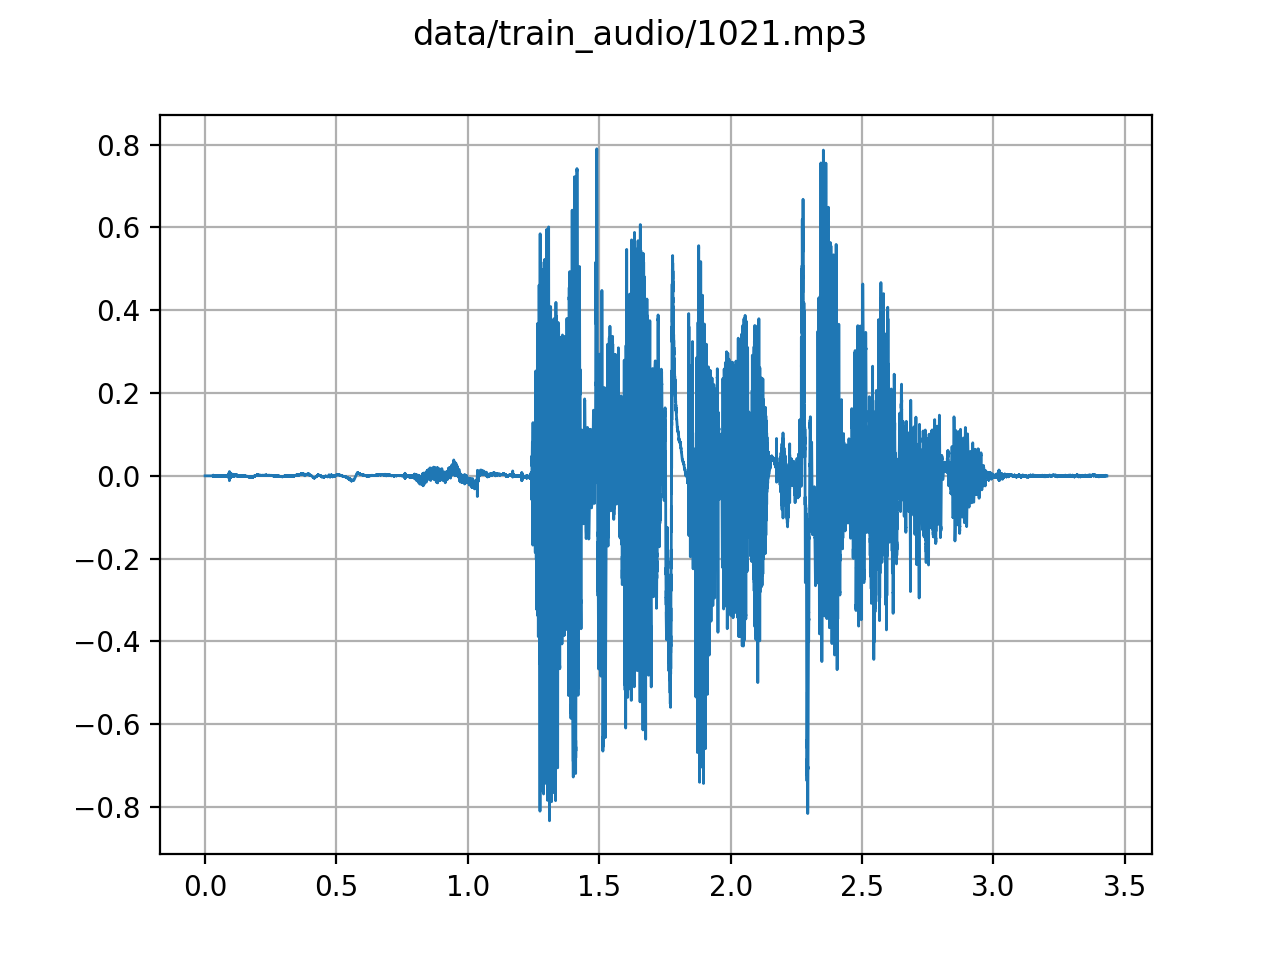
\includegraphics[width=\textwidth]{joeynmt-speech2text/images/1021_Eine_Beleuchtung_ist_vorgeschrieben_Waveform.png}
        \caption{Waveform}
        \label{fig:1021_waveform}
    \end{subfigure}
     \hfill
    \begin{subfigure}[b]{0.32\textwidth}
        \centering
        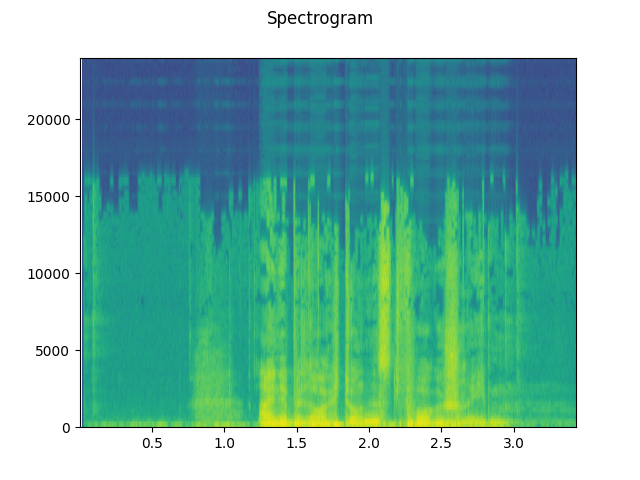
\includegraphics[width=\textwidth]{joeynmt-speech2text/images/1021_Eine_Beleuchtung_ist_vorgeschrieben_Spectrogram.png}
        \caption{Spectrogramm}
        \label{fig:1021_spectrogramm}
    \end{subfigure}
     \hfill
    \begin{subfigure}[b]{0.32\textwidth}
        \centering
        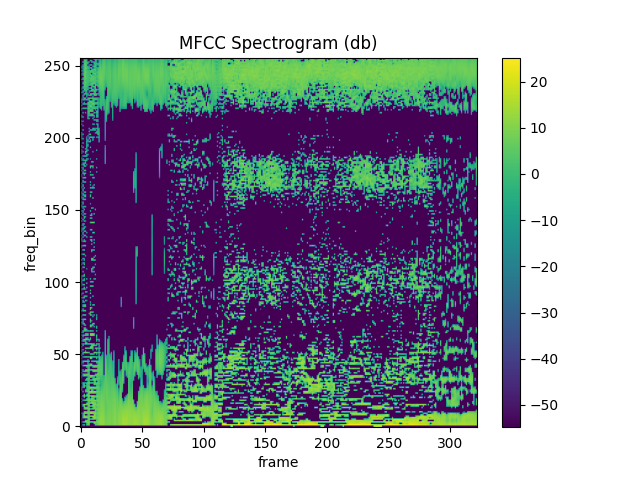
\includegraphics[width=\textwidth]{joeynmt-speech2text/images/1021_Eine_Beleuchtung_ist_vorgeschrieben_MFCC.png}
        \caption{MFCC}
        \label{fig:1021_mfcc}
    \end{subfigure}
    \caption{Visualizations of \enquote{Eine Beleuchtung ist vorgeschrieben.}}
    \label{fig:beleuchtung_viz}
\end{figure*}

\subsection{Dataset}

The dataset used throughout this paper is the open \enquote{Common Voice Corpus 7.0} dataset by Mozilla~\cite{commonvoice:2020}.
We have chosen the German language as that's what the authors are most familiar with which allows us to better evaluate the dataset quality.
The unprocessed dataset contains 26\,GB of audio files which 1035\,h according to \enquote{Common Voice}.

After listening to few audio files, the authors decided to filter the dataset for one major reason:
There were audio files that had accents that made it hard to understand even for native speakers.

Furthermore, even though the authors think that enterprise speech to text models
should handle accents as well as differences between male and female voices,
we decided that it would be out-of-scope for this paper.
Therefore, all audio files were filtered according to these rules:

\begin{itemize}
    \item max. 75 characters
    \item no accent and no Swiss- or Austrian-German
    \item male voice
    \item no special characters in the corresponding text
\end{itemize}

Having these limitations makes it easier to rule out issues during evaluation.

However, these limitations yield only about 7500 audio files for training and around 100 for testing and evaluation.  On top of this, the quality of audio files still differs enormously.  Whereas some have crystal clear voices, other have lot of noise and even contain mouse-click or keyboard sounds.


\section{Results and Discussion}


\bibliography{acl2020}
\bibliographystyle{acl_natbib}

\appendix

\section{Appendices}
TODO

\section{Supplemental Material}
\label{sec:supplemental}
TODO

\end{document}
